\documentclass[11pt,oneside,a4paper]{article}
\usepackage{graphicx}
\usepackage{booktabs}
\usepackage{caption}
\usepackage{subcaption}
\usepackage{amsmath}
\usepackage{amsfonts}
\usepackage{amssymb}
\usepackage{lscape}
\usepackage{psfrag}
\usepackage[usenames]{color}
\usepackage{bbm}
\usepackage[update]{epstopdf}
\usepackage[bookmarks,pdfstartview=FitH,a4paper,pdfborder={0 0 0}]{hyperref}
\usepackage{verbatim}
\usepackage{listings}
\usepackage{textcomp}
\usepackage{course}
\usepackage{fancyhdr}
\usepackage{multirow}
\pagestyle{fancy}
\usepackage{tikz}
\usepackage{subcaption} 

\renewcommand{\sectionmark}[1]{\markboth{#1}{#1}}
\renewcommand{\subsectionmark}[1]{\markright{#1}}

\fancyhf{}
\fancyhead[RO]{\nouppercase{\footnotesize\sc\leftmark\ \hrulefill\ \thepage}}
\fancyhead[RE]{\nouppercase{\footnotesize\sc\thepage\ \hrulefill\ }}
\renewcommand{\headrulewidth}{0pt}

\makeatletter
\def\cleardoublepage{\clearpage\if@twoside \ifodd\c@page\else%
\hbox{}%
\thispagestyle{empty}%
\clearpage%
\if@twocolumn\hbox{}\clearpage\fi\fi\fi}
\makeatother


\renewcommand{\topfraction}{0.9}  % max fraction of floats at top
\renewcommand{\bottomfraction}{0.8} % max fraction of floats at bottom
% Parameters for TEXT pages (not float pages):
\setcounter{topnumber}{2}
\setcounter{bottomnumber}{2}
\setcounter{totalnumber}{4}            % 2 may work better
\setcounter{dbltopnumber}{2}           % for 2-column pages
\renewcommand{\dbltopfraction}{0.9}    % fit big float above 2-col. text
\renewcommand{\textfraction}{0.07}     % allow minimal text w. figs
% Parameters for FLOAT pages (not text pages):
\renewcommand{\floatpagefraction}{0.7}  % require fuller float pages
% N.B.: floatpagefraction MUST be less than topfraction !!
\renewcommand{\dblfloatpagefraction}{0.7} % require fuller float pages

\sloppy

\widowpenalty=10000
\clubpenalty=10000

\edef\today{%\number\day\
\ifcase\month\or
January\or February\or March\or April\or May\or June\or July\or
August\or September\or October\or November\or December\fi\ \number\year}
\title{\vspace*{40.0mm}
  \bf\sf Support Vector Machine Assignment 
         \vspace*{20.0mm} \\
  \vspace*{40.0mm}
  %\vspace{-20mm}\framebox{DRAFT VERSION}\vspace{20mm} \\
  }
\author{\sf Mohamedhakim Elakhrass}
\date{\sf 15/07/2016}

\begin{document}

\begin{figure}
  \parbox[t]{125mm}{
    \vspace*{6mm}
    \scriptsize\sf           FACULTY OF BIOSCIENCE ENGINEERING\\
    \scriptsize\sf           Masters of Bioinformatics \\
    \scriptsize\sf\bfseries  Support Vector Machines \\}
  \parbox[t]{40mm}{
    \begin{flushright}
      \includegraphics[height=15mm]{logo.eps}
    \end{flushright}}
\end{figure}

\maketitle
\thispagestyle{empty}
\raggedbottom

\cleardoublepage
\pagenumbering{roman}
\setcounter{tocdepth}{2}
\tableofcontents
\cleardoublepage
\pagenumbering{arabic}

\cleardoublepage

\section{Objectives}
The objectives of this assignment are to learn and work with real life applications of SVM. 
\section{Simple 2 Gaussian}
This sections looks at two simulated datasets. The datasets are created using the MatLab $randn()$ function. One dataset is centered around (1,1) and the other (-1,1)\\

\begin{figure}[h!]
	\begin{subfigure}[b]{0.4\textwidth}
		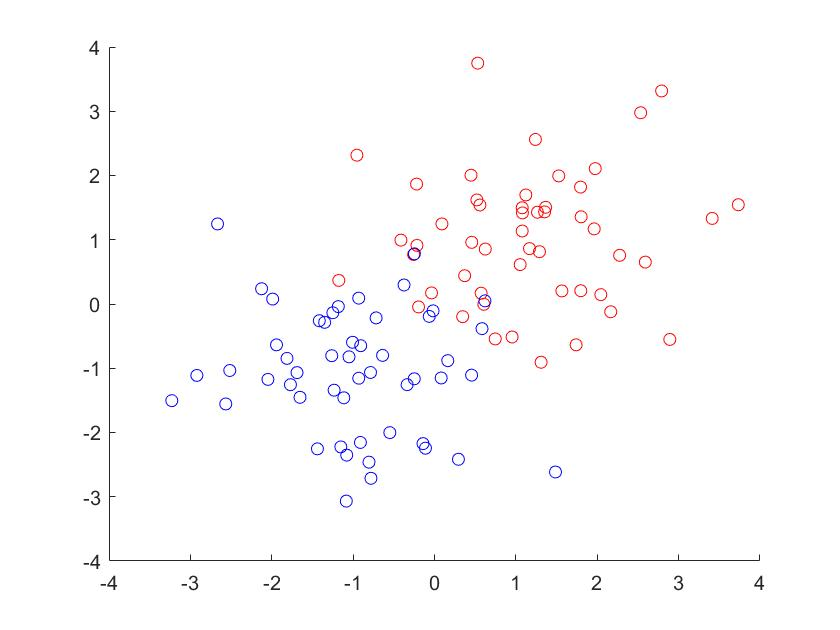
\includegraphics[width=\textwidth]{../Figures/2_Gaussians}
		\caption{Two Gaussians}
		\label{fig:1}
	\end{subfigure}
	%
	\begin{subfigure}[b]{0.4\textwidth}
		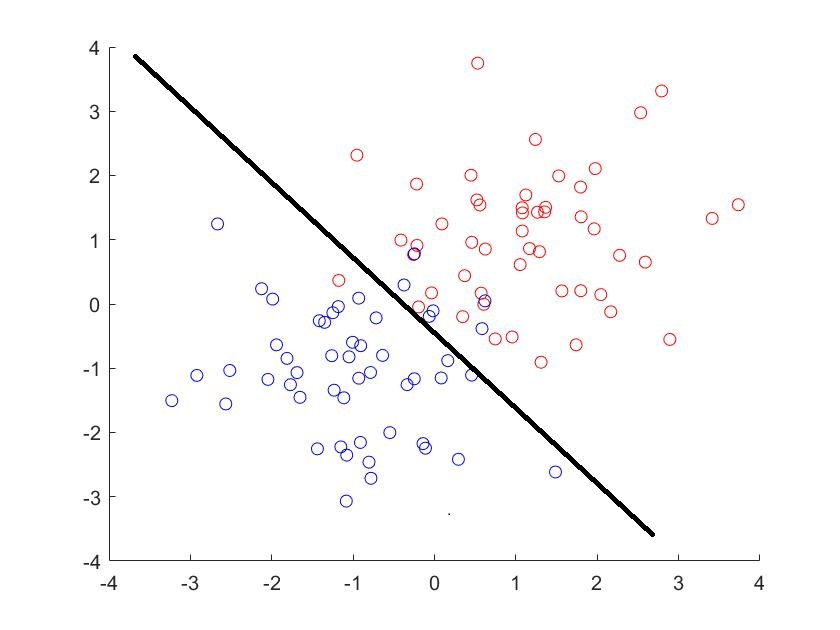
\includegraphics[width=\textwidth]{../Figures/2_Gaussians_with_classifier}
		\caption{Two Gaussians with optimal classifier}
		\label{fig:2}
	\end{subfigure}
\end{figure}
Figure 1: (a) Two Simulated Datasets. (b) Two Simulated Datasets with Optimal Classifier.\\

\textbf{Given this figure, can you make a geometric construction using lines to estimate the optimal classifier? Under which conditions do you think this construction is optimal/valid?}\\

Figure 1:a is the output of the simulated datasets. As shown in figure 1:b it is possible to show an optimal classifier. This classifier is known as the Bayes Classifier. A test observation is assigned with predictor vector $x_{0}$ to the class j for which    \[ Pr(Y=j|X=x_{0}) \] is largest. The classifier is optimal because it produces the lowest possible error rate and allows for some overlap. The classifier is valid because the underlying distribution of the dataset is known. 

\section{The Support Vector Machine}
\end{document}